\documentclass[a4paper, 12pt]{article}
\usepackage{geometry}
\geometry{verbose,a4paper,tmargin=2cm,bmargin=2cm,lmargin=2cm,rmargin=2cm}
\usepackage[T2A]{fontenc}
\usepackage[utf8]{inputenc}
\usepackage[english,russian]{babel}
\newif\ifisinsp
\newif\ifisone
\newif\ifisname
\isinsptrue
\isonetrue
\isnamefalse
\def \labtype {Лабораторная}
% Это для нумерации страниц после титульника
\usepackage{fancyhdr}
\pagestyle{fancy}
\renewcommand{\headrulewidth}{0pt}
\fancyfoot[C] {\thepage}

\usepackage{hyperref}
\hypersetup{pdftex,colorlinks=true,allcolors=black}
\usepackage{hypcap}

\usepackage{graphicx}
\usepackage{adjustbox}
\usepackage{multirow}

\def \labnum {1}
\def \labtype {Домашняя}
\def \labsubj {Моделирование}
\def \labauthor {Чебыкин И. Б.}
\def \labgroup {P3301}
\def \labinsp {Муравьева-Витковская Л. А.}
\def \labname {Вариант: 23/5}
% https://en.wikibooks.org/wiki/LaTeX/Source_Code_Listings
\usepackage{listings}
\usepackage{color}
\definecolor{mygreen}{rgb}{0,0.6,0}
\definecolor{mygray}{rgb}{0.5,0.5,0.5}
\definecolor{mymauve}{rgb}{0.58,0,0.82}
\definecolor{lightgray}{rgb}{.9,.9,.9}
\definecolor{darkgray}{rgb}{.4,.4,.4}
\definecolor{purple}{rgb}{0.65, 0.12, 0.82}

\lstdefinelanguage{JavaScript}{
  keywords={typeof, new, true, false, catch, function, return, null, catch, switch, var, if, in, while, do, else, case, break},
  keywordstyle=\ttfamily\color{blue}\bfseries,
  ndkeywords={class, export, boolean, throw, implements, import, this},
  ndkeywordstyle=\ttfamily\color{darkgray}\bfseries,
  identifierstyle=\ttfamily\color{black},
  sensitive=false,
  comment=[l]{//},
  morecomment=[s]{/*}{*/},
  commentstyle=\color{purple}\ttfamily,
  stringstyle=\color{red}\ttfamily,
  morestring=[b]',
  morestring=[b]"
}


\lstdefinelanguage{CSS}{
  morekeywords={accelerator,azimuth,background,background-attachment,
    background-color,background-image,background-position,
    background-position-x,background-position-y,background-repeat,
    behavior,border,border-bottom,border-bottom-color,
    border-bottom-style,border-bottom-width,border-collapse,
    border-color,border-left,border-left-color,border-left-style,
    border-left-width,border-right,border-right-color,
    border-right-style,border-right-width,border-spacing,
    border-style,border-top,border-top-color,border-top-style,
    border-top-width,border-width,bottom,caption-side,clear,
    clip,color,content,counter-increment,counter-reset,cue,
    cue-after,cue-before,cursor,direction,display,elevation,
    empty-cells,filter,float,font,font-family,font-size,
    font-size-adjust,font-stretch,font-style,font-variant,
    font-weight,height,ime-mode,include-source,
    layer-background-color,layer-background-image,layout-flow,
    layout-grid,layout-grid-char,layout-grid-char-spacing,
    layout-grid-line,layout-grid-mode,layout-grid-type,left,
    letter-spacing,line-break,line-height,list-style,
    list-style-image,list-style-position,list-style-type,margin,
    margin-bottom,margin-left,margin-right,margin-top,
    marker-offset,marks,max-height,max-width,min-height,
    min-width,-moz-binding,-moz-border-radius,
    -moz-border-radius-topleft,-moz-border-radius-topright,
    -moz-border-radius-bottomright,-moz-border-radius-bottomleft,
    -moz-border-top-colors,-moz-border-right-colors,
    -moz-border-bottom-colors,-moz-border-left-colors,-moz-opacity,
    -moz-outline,-moz-outline-color,-moz-outline-style,
    -moz-outline-width,-moz-user-focus,-moz-user-input,
    -moz-user-modify,-moz-user-select,orphans,outline,
    outline-color,outline-style,outline-width,overflow,
    overflow-X,overflow-Y,padding,padding-bottom,padding-left,
    padding-right,padding-top,page,page-break-after,
    page-break-before,page-break-inside,pause,pause-after,
    pause-before,pitch,pitch-range,play-during,position,quotes,
    -replace,richness,right,ruby-align,ruby-overhang,
    ruby-position,-set-link-source,size,speak,speak-header,
    speak-numeral,speak-punctuation,speech-rate,stress,
    scrollbar-arrow-color,scrollbar-base-color,
    scrollbar-dark-shadow-color,scrollbar-face-color,
    scrollbar-highlight-color,scrollbar-shadow-color,
    scrollbar-3d-light-color,scrollbar-track-color,table-layout,
    text-align,text-align-last,text-decoration,text-indent,
    text-justify,text-overflow,text-shadow,text-transform,
    text-autospace,text-kashida-space,text-underline-position,top,
    unicode-bidi,-use-link-source,vertical-align,visibility,
    voice-family,volume,white-space,widows,width,word-break,
    word-spacing,word-wrap,writing-mode,z-index,zoom},
  morestring=[s]{:}{;},
  sensitive,
  morecomment=[s]{/*}{*/}
}

% злостный костылище
% http://roman.khimov.ru/2011/05/19/latex-listings-cyrillic/
\lstset{
literate={а}{{\selectfont\char224}}1
{б}{{\selectfont\char225}}1
{в}{{\selectfont\char226}}1
{г}{{\selectfont\char227}}1
{д}{{\selectfont\char228}}1
{е}{{\selectfont\char229}}1
{ё}{{\"e}}1
{ж}{{\selectfont\char230}}1
{з}{{\selectfont\char231}}1
{и}{{\selectfont\char232}}1
{й}{{\selectfont\char233}}1
{к}{{\selectfont\char234}}1
{л}{{\selectfont\char235}}1
{м}{{\selectfont\char236}}1
{н}{{\selectfont\char237}}1
{о}{{\selectfont\char238}}1
{п}{{\selectfont\char239}}1
{р}{{\selectfont\char240}}1
{с}{{\selectfont\char241}}1
{т}{{\selectfont\char242}}1
{у}{{\selectfont\char243}}1
{ф}{{\selectfont\char244}}1
{х}{{\selectfont\char245}}1
{ц}{{\selectfont\char246}}1
{ч}{{\selectfont\char247}}1
{ш}{{\selectfont\char248}}1
{щ}{{\selectfont\char249}}1
{ъ}{{\selectfont\char250}}1
{ы}{{\selectfont\char251}}1
{ь}{{\selectfont\char252}}1
{э}{{\selectfont\char253}}1
{ю}{{\selectfont\char254}}1
{я}{{\selectfont\char255}}1
{А}{{\selectfont\char192}}1
{Б}{{\selectfont\char193}}1
{В}{{\selectfont\char194}}1
{Г}{{\selectfont\char195}}1
{Д}{{\selectfont\char196}}1
{Е}{{\selectfont\char197}}1
{Ё}{{\"E}}1
{Ж}{{\selectfont\char198}}1
{З}{{\selectfont\char199}}1
{И}{{\selectfont\char200}}1
{Й}{{\selectfont\char201}}1
{К}{{\selectfont\char202}}1
{Л}{{\selectfont\char203}}1
{М}{{\selectfont\char204}}1
{Н}{{\selectfont\char205}}1
{О}{{\selectfont\char206}}1
{П}{{\selectfont\char207}}1
{Р}{{\selectfont\char208}}1
{С}{{\selectfont\char209}}1
{Т}{{\selectfont\char210}}1
{У}{{\selectfont\char211}}1
{Ф}{{\selectfont\char212}}1
{Х}{{\selectfont\char213}}1
{Ц}{{\selectfont\char214}}1
{Ч}{{\selectfont\char215}}1
{Ш}{{\selectfont\char216}}1
{Щ}{{\selectfont\char217}}1
{Ъ}{{\selectfont\char218}}1
{Ы}{{\selectfont\char219}}1
{Ь}{{\selectfont\char220}}1
{Э}{{\selectfont\char221}}1
{Ю}{{\selectfont\char222}}1
{Я}{{\selectfont\char223}}1
}
\lstset{ %
	backgroundcolor=\color{white},   % choose the background color; you must add \usepackage{color} or \usepackage{xcolor}
	basicstyle=\ttfamily\footnotesize,        % the size of the fonts that are used for the code
	breakatwhitespace=false,         % sets if automatic breaks should only happen at whitespace
	breaklines=true,                 % sets automatic line breaking
	captionpos=b,                    % sets the caption-position to bottom
	commentstyle=\color{black},    % comment style
	deletekeywords={...},            % if you want to delete keywords from the given language
	escapeinside={\%*}{*)},          % if you want to add LaTeX within your code
	extendedchars=true,              % lets you use non-ASCII characters; for 8-bits encodings only, does not work with UTF-8
	keepspaces=true,                 % keeps spaces in text, useful for keeping indentation of code (possibly needs columns=flexible)
	keywordstyle=\color{blue},       % keyword style
	language=Octave,                 % the language of the code
	otherkeywords={*,...},            % if you want to add more keywords to the set
	rulecolor=\color{black},         % if not set, the frame-color may be changed on line-breaks within not-black text (e.g. comments (green here))
	showspaces=false,                % show spaces everywhere adding particular underscores; it overrides 'showstringspaces'
	showstringspaces=false,          % underline spaces within strings only
	showtabs=false,                  % show tabs within strings adding particular underscores
	stepnumber=2,                    % the step between two line-numbers. If it's 1, each line will be numbered
	stringstyle=\color{mymauve},     % string literal style
	tabsize=2,	                   % sets default tabsize to 2 spaces
}

\isnametrue
\lstset{
	caption=\lstname,
	basicstyle=\ttfamily\selectfont\scriptsize
}
\begin{document}
\begin{titlepage}
	\begin{center}
		\large
		Университет ИТМО

		\vspace{0.25cm}
		
		Факультет программной инженерии и компьютерной техники
		
		Кафедра вычислительной техники
		\vfill
		
		\textsc{\labtype\spaceработа \ifisnum № \labnum{} \fi по дисциплине \\"\labsubj" \ifisname\small \\ \labname \fi}
			
		\bigskip
	\end{center}
	\vfill
	\vfill
	
	\begin{flushright}
	\ifisone
	Выполнил: \labauthor
	\else
	Выполнили: \labauthor
	\fi

	\vspace{0.25cm}
	Группа: \labgroup
			
	\vspace{0.25cm}
	\ifisinsp
	Проверяющий: \labinsp
	\fi
	\end{flushright}
	\vfill
	
	\begin{center}
	СПб, \the\year
	\end{center}
\end{titlepage}

\tableofcontents
\newpage
\section{Цель работы}
Изучение метода Марковских случайных процессов и его
применение для исследования простейших моделей – систем массового
обслуживания (СМО) с однородным потоком заявок.
\section{Задание}
Разработка и расчет Марковских моделей одно- и многоканальных
СМО с однородным потоком заявок и выбор наилучшего варианта
построения СМО в соответствии с заданным критерием эффективности.
\subsection{Этапы задания}
\begin{enumerate}
	\item Разработка Марковских моделей исследуемых систем.
	\item Освоение программы по расчету Марковских моделей.
	\item Проведение расчетов по разработанным моделям и обработка результатов.
	\item Анализ полученных результатов.
	\item Выбор наилучшего варианта организации системы
\end{enumerate}

\section{Выполнение}
\subsection{Параметры}

\subsubsection{Параметры структурной и функциональной организации систем}

\begin{tabular}{|c|c|c|c|c|}
\hline
\multicolumn{2}{|c|}{Система 1} & \multicolumn{2}{c|}{Система 2} & \multirow{2}{*}{Критерий эффективности} \\ \cline{1-4}
П             & ЕН              & П            & ЕН              &                                         \\ \hline
2             & 0/2             & 3            & 0/0/2           & максимальная загрузка системы           \\ \hline
\end{tabular}

\subsubsection{Параметры структурной и функциональной организации систем}

\begin{tabular}{|c|c|c|c|c|}
\hline
Интенс. потока  & Ср. длит. обслуж. & \multicolumn{3}{c|}{Вероятности занятия прибора} \\ \hline
$\lambda$ (1/c) & B (c)             & П1             & П2             & П3             \\ \hline
0.5             & 10                & 0.5            & 0.4            & 0.1            \\ \hline
\end{tabular}
\\

\newpage
\subsection{Система 1}
\includegraphics[width=200px]{img/s1.png}

$p_1 = 0.5, p_2 = 0.5$

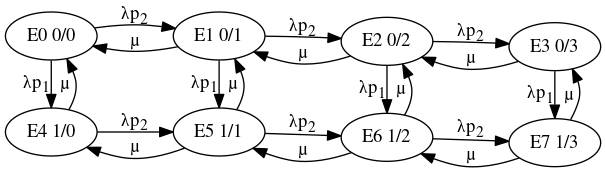
\includegraphics[resolution=128]{img/g1.png}

\subsubsection{Стационарные вероятности состояний}

\begin{tabular}{|l|l|}
\hline
Код состояния & Вероятность \\ \hline
E0            & 0.0113      \\ \hline
E1            & 0.0281      \\ \hline
E2            & 0.0704      \\ \hline
E3            & 0.1759      \\ \hline
E4            & 0.0281      \\ \hline
E5            & 0.0704      \\ \hline
E6            & 0.1759      \\ \hline
E7            & 0.4398      \\ \hline
\end{tabular}

\subsubsection{Характеристики системы 1}
\begin{tabular}{|c|c|c|c|}
\hline
Характеристика                      & Прибор & Расчетная формула                                                       & Значение \\ \hline
\multirow{3}{*}{Нагрузка}           & П1     & $y_1 = \lambda\cdot b\cdot b p_1$                                       & 2,5      \\ \cline{2-4}
                                    & П2     & $y_2 = \lambda\cdot b\cdot b p_2$                                       & 2,5      \\ \cline{2-4}
                                    & Сумма  & $y = y_1 + y_2$                                                         & 5        \\ \hline
\multirow{3}{*}{Загрузка}           & П1     & $\rho_1 = p_4 + p_5 + p_6 + p_7$                                        & 0,7142   \\ \cline{2-4}
                                    & П2     & $\rho_2 = p_1 + p_2 + p_3 + p_5 + p_6 + p_7$                            & 0,9605   \\ \cline{2-4}
                                    & Сумма  & $\rho = \frac{\rho_1 + \rho_2}{2}$                                      & 0,83735  \\ \hline
\multirow{3}{*}{Длина очереди}      & П1     & $l_1 = 0$                                                               & 0        \\ \cline{2-4}
                                    & П2     & $l_2 = p_2 + 2p_3 + p_6 + 2p_7$                                         & 1,4777   \\ \cline{2-4}
                                    & Сумма  & $l = l_2$                                                               & 1,4777   \\ \hline
\multirow{3}{*}{Число заявок}       & П1     & $m_1 = p_4 + p_5 + p_6 + p_7$                                           & 0,9671   \\ \cline{2-4}
                                    & П2     & $m_2 = p1 + 2p_2 + 3p_3 + p_5 + 2p_6 + 3p_7$                            & 3,9583   \\ \cline{2-4}
                                    & Сумма  & $m = m_1 + m_2$                                                         & 4,9254   \\ \hline
\multirow{3}{*}{Время ожидания}     & П1     & $w_1=\frac{l_1}{\lambda'_1}$                                            & 0        \\ \cline{2-4}
                                    & П2     & $w_2=\frac{l_2}{\lambda'_2}$                                            & 15,3815  \\ \cline{2-4}
                                    & Сумма  & $w = \frac{\lambda'_1 w_1}{\lambda'} + \frac{\lambda'_2 w_2}{\lambda'}$ & 8,8168   \\ \hline
\multirow{3}{*}{Время пребывания}   & П1     & $u_1 = \frac{m_1}{\lambda'_1}$                                          & 13,5353  \\ \cline{2-4}
                                    & П2     & $u_2 = \frac{m_2}{\lambda'_2}$                                          & 41,2022  \\ \cline{2-4}
                                    & Сумма  & $u = \frac{m}{\lambda'}$                                                & 29,3878  \\ \hline
\multirow{3}{*}{Вероятность потери} & П1     & $\pi_1 = p_4 + p_5 + p_6 + p_7$                                         & 0,7142   \\ \cline{2-4}
                                    & П2     & $\pi_2 = p_3 + p_7$                                                     & 0,6157   \\ \cline{2-4}
                                    & Сумма  & $\pi = q_1 \cdot \pi_1 + q_2 \cdot \pi_2$                               & 0,66495  \\ \hline
\multirow{3}{*}{Производительность} & П1     & $\lambda'_1 = \lambda \cdot q_1(1 - \pi_1)$                             & 0,07145  \\ \cline{2-4}
                                    & П2     & $\lambda'_2 = \lambda \cdot q_2(1 - \pi_2)$                             & 0,09607  \\ \cline{2-4}
                                    & Сумма  & $\lambda' = \lambda \cdot (1 - \pi)$                                    & 0,1676   \\ \hline
\end{tabular}

\newpage
\subsection{Система 2}
\includegraphics[width=200px]{img/s2.png}

$p_1 = 0.5, p_2 = 0.4, p_3 = 0.1$\\

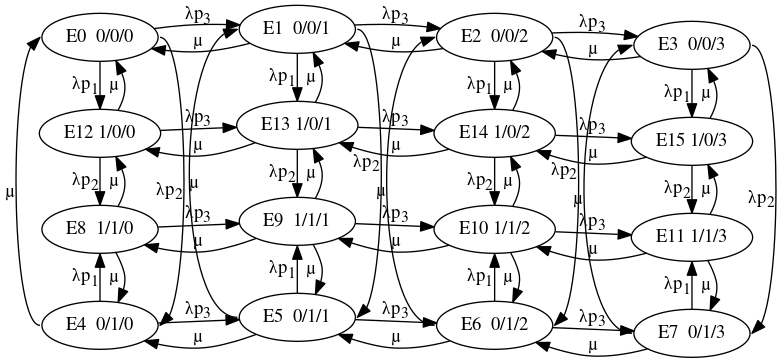
\includegraphics[resolution=128]{img/g2.png}

\subsubsection{Стационарные вероятности состояний}

\begin{tabular}{|l|l|}
\hline
Код состояния & Вероятность \\ \hline
E0            & 0.2962      \\ \hline
E1            & 0.1481      \\ \hline
E2            & 0.0740      \\ \hline
E3            & 0.0370      \\ \hline
E4            & 0.1481      \\ \hline
E5            & 0.0740      \\ \hline
E6            & 0.0370      \\ \hline
E7            & 0.0185      \\ \hline
E8            & 0.0592      \\ \hline
E9            & 0.0296      \\ \hline
E10           & 0.0148      \\ \hline
E11           & 0.0074      \\ \hline
E12           & 0.0296      \\ \hline
E13           & 0.0148      \\ \hline
E14           & 0.0074      \\ \hline
E15           & 0.0037      \\ \hline
\end{tabular}

\subsubsection{Характеристики системы 2}
\begin{adjustbox}{max width=\textwidth}
\begin{tabular}{|c|c|c|c|}
\hline
Характеристика                      & Прибор & Расчетная формула                                                                                        & Значение \\ \hline
\multirow{4}{*}{Нагрузка}           & П1     & $y_1 = \lambda\cdot b\cdot b p_1$                                                                        & 2,5      \\ \cline{2-4}
                                    & П2     & $y_2 = \lambda\cdot b\cdot b p_2$                                                                        & 2        \\ \cline{2-4}
                                    & П3     & $y_3 = \lambda\cdot b\cdot b p_3$                                                                        & 0.5      \\ \cline{2-4}
                                    & Сумма  & $y = y_1 + y_2 + y_3$                                                                                    & 5        \\ \hline
\multirow{4}{*}{Загрузка}           & П1     & $\rho_1 = p_8 + p_9 + p_{10} + p_{11} + p_{12} + p_{13} + p_{14} + p_{15}$                                           & 0,1665   \\ \cline{2-4}
                                    & П2     & $\rho_2 = p_4 + p_5 + p_6 + p_7 + p_8 + p_9 + p_{10} + p_{11}$                                               & 0,3886   \\ \cline{2-4}
                                    & П3     & $\rho_3 = p_1 + p_2 + p_3 + p_5 + p_6 + p_7 + p_9 + p_{10} + p_{11} + p_{13} + p_{14} + p_{15}$                    & 0,4663   \\ \cline{2-4}
                                    & Сумма  & $\rho = \frac{\rho_1 + \rho_2 + \rho_3}{3}$                                                              & 0,34046  \\ \hline
\multirow{4}{*}{Длина очереди}      & П1     & $l_1 = 0$                                                                                                & 0        \\ \cline{2-4}
                                    & П2     & $l_2 = 0$                                                                                                & 0        \\ \cline{2-4}
                                    & П3     & $l_3 = p_2 + 2p_3 + p_6 + 2p_7 + p_{10} + 2p_{11} + p_{14} + 2p_{15}$                                            & 0,2664   \\ \cline{2-4}
                                    & Сумма  & $l = l_3$                                                                                                & 0,2664   \\ \hline
\multirow{4}{*}{Число заявок}       & П1     & $m_1 = p_8+p_9+p_{10}+p_{11}+p_{12}+p_{13}+p_{14}+p_{15}$                                                            & 0,1665   \\ \cline{2-4}
                                    & П2     & $m_2 = p_4+p_5+p_6+p_7+p_8+p_9+p_{10}+p_{11}$                                                                & 0,3886   \\ \cline{2-4}
                                    & П3     & $m_3 = p_1 + 2p_2+3p_3 + p_5 + 2p_6 + 3p_7 + p9+ 2p_{10} + 3p_{11} + p_{13} + 2p_{14} + 3p_{15}$                   & 0,7327   \\ \cline{2-4}
                                    & Сумма  & $m = m_1 + m_2 + m_3$                                                                                    & 1,2878   \\ \hline
\multirow{4}{*}{Время ожидания}     & П1     & $w_1=\frac{l_1}{\lambda'_1}$                                                                             & 0        \\ \cline{2-4}
                                    & П2     & $w_2=\frac{l_2}{\lambda'_2}$                                                                             & 0        \\ \cline{2-4}
                                    & П3     & $w_3=\frac{l_3}{\lambda'_3}$                                                                             & 5,70816  \\ \cline{2-4}
                                    & Сумма  & $w = \frac{\lambda'_1 w_1}{\lambda'} + \frac{\lambda'_2 w_2}{\lambda'}+ \frac{\lambda'_3 w_3}{\lambda'}$ & 0,70602  \\ \hline
\multirow{4}{*}{Время пребывания}   & П1     & $u_1 = \frac{m_1}{\lambda'_1}$                                                                           & 0,7990   \\ \cline{2-4}
                                    & П2     & $u_2 = \frac{m_2}{\lambda'_2}$                                                                           & 3,1780   \\ \cline{2-4}
                                    & П3     & $u_3 = \frac{m_3}{\lambda'_3}$                                                                           & 15,6996  \\ \cline{2-4}
                                    & Сумма  & $u = \frac{m}{\lambda'}$                                                                                 & 3,4130   \\ \hline
\multirow{4}{*}{Вероятность потери} & П1     & $\pi_1 = p_8+p_9+p_{10}+p_{11}+p_{12}+p_{13}+p_{14}+p_{15}$                                                          & 0,1665   \\ \cline{2-4}
                                    & П2     & $\pi_2 = p_4+p_5+p_6+p_7+p_8+p_9+p_{10}+p_{11}$                                                              & 0,3886   \\ \cline{2-4}
                                    & П3     & $\pi_3 = p_3 + p_7 + p_{11} + p_{15}$                                                                        & 0,0666   \\ \cline{2-4}
                                    & Сумма  & $\pi = q_1 \cdot \pi_1 + q_2 \cdot \pi_2 + q_3 \cdot \pi_3$                                              & 0,24535  \\ \hline
\multirow{4}{*}{Производительность} & П1     & $\lambda'_1 = \lambda \cdot q_1(1 - \pi_1)$                                                              & 0,208375 \\ \cline{2-4}
                                    & П2     & $\lambda'_2 = \lambda \cdot q_2(1 - \pi_2)$                                                              & 0,12228  \\ \cline{2-4}
                                    & П3     & $\lambda'_3 = \lambda \cdot q_3(1 - \pi_3)$                                                              & 0,04667  \\ \cline{2-4}
                                    & Сумма  & $\lambda' = \lambda \cdot (1 - \pi)$                                                                     & 0,377325 \\ \hline
\end{tabular}
\end{adjustbox}

\section{Вывод}
Исходя из заданного критерия эффективности по максимальной загрузке системы,
система 1 со значением 0,83735 эффективнее системы 2 со значением 0,34046.
\end{document}
